% !TeX spellcheck = en_US
\documentclass{beamer}
\usepackage{Tsinghua}
\usepackage{graphicx}
\usepackage{amsmath, amssymb}
\usefonttheme{serif}
\usepackage{siunitx}
\usepackage{latexsym,amsmath,xcolor,multicol,booktabs,calligra}
\usepackage{graphicx,pstricks,listings,stackengine}
\title{Heat Transfer in TPMS-structures}
\subtitle[]{Final Presentation}
\institute{Dept. of Mechanical Engineering}
\author{Axel Fritz \& You Ming}
\date{Monday June 8th 2026}
\newcommand{\happy}{:)}
\newcommand{\sad}{:(}
\def\cmd#1{\texttt{\color{red}\footnotesize $\backslash$#1}}
\def\env#1{\texttt{\color{blue}\footnotesize #1}}
\definecolor{deepblue}{rgb}{0,0,0.5}
\definecolor{deepred}{rgb}{0.6,0,0}
\definecolor{deepgreen}{rgb}{0,0.5,0}
\definecolor{halfgray}{gray}{0.55}
\lstset{
	basicstyle=\ttfamily\small,
	keywordstyle=\bfseries\color{deepblue},
	emphstyle=\ttfamily\color{deepred},    % Custom highlighting style
	stringstyle=\color{deepgreen},
	numbers=left,
	numberstyle=\small\color{halfgray},
	rulesepcolor=\color{red!20!green!20!blue!20},
	frame=shadowbox,
}
\AtBeginSection[]
{
	\begin{frame}
		\frametitle{Table of Contents}
		\tableofcontents[currentsection]
	\end{frame}
}
\begin{document}

\begin{frame}
	\titlepage
	\begin{figure}[htpb]
		\begin{center}
			
\includegraphics[width=0.2\linewidth]{Tsinghua_University_Logo.eps}
		\end{center}
	\end{figure}
\end{frame}
\begin{frame}
	\frametitle{Table of Contents}
	\tableofcontents
\end{frame}
\section{Background}

	\begin{frame}{Heat Exchangers}
		Physical models:
		\begin{itemize}
			\item Fluid dynamics (Navier-Stokes eqns.)
			\item Heat conduction (Heat eqn.)
		\end{itemize}

		
		
		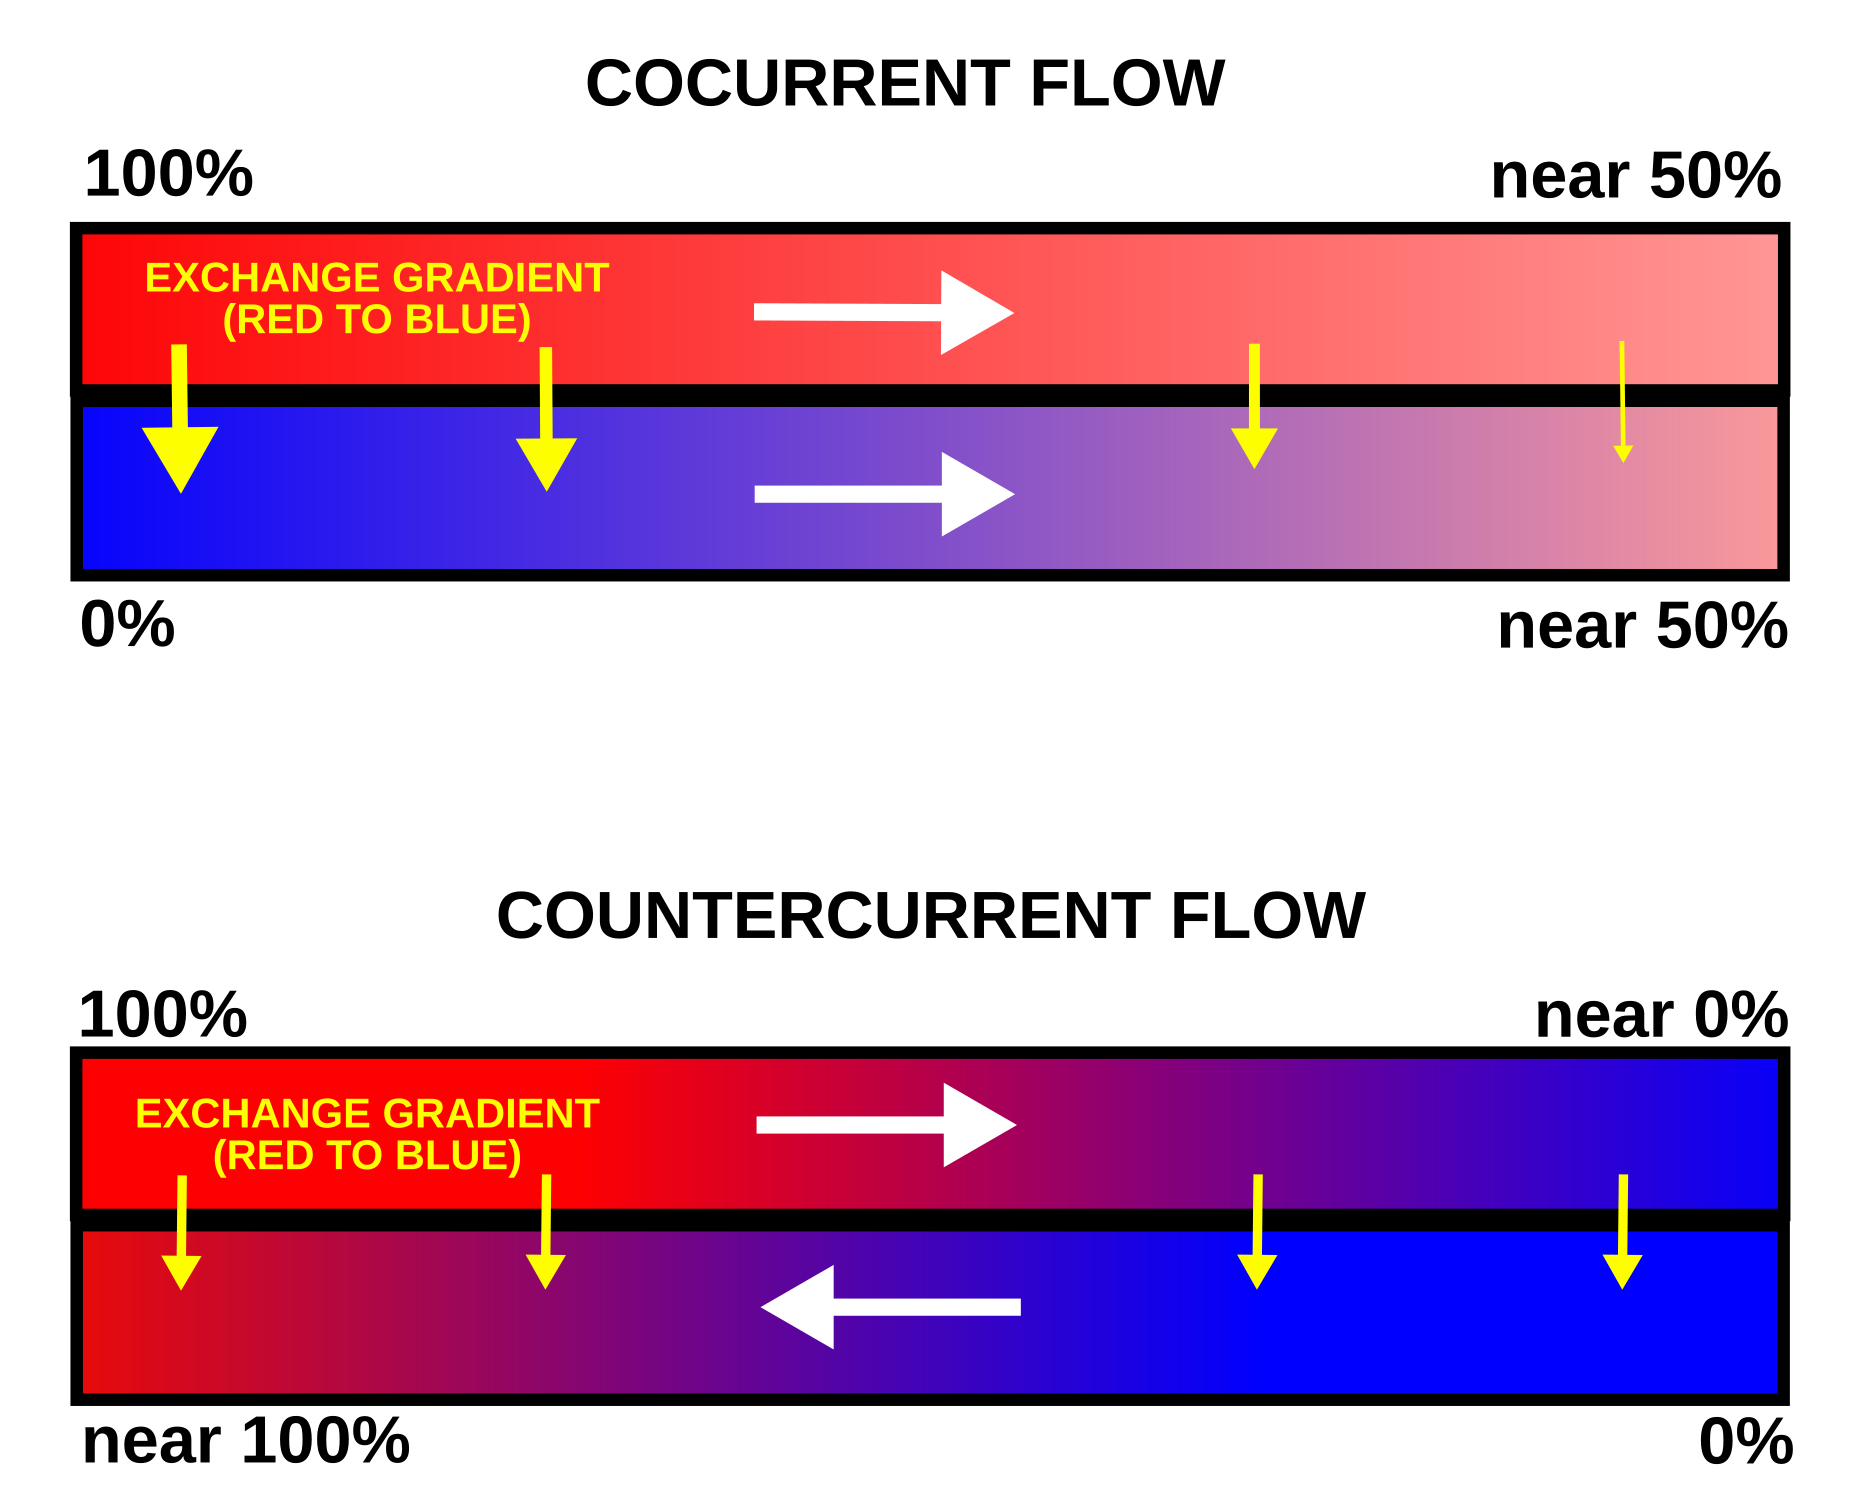
\includegraphics[width=0.45\textwidth]{imgs/heatdiagram.png}
	\end{frame}
	\begin{frame}{Introduction}
		How is it justified to write an entire project about something so simple and well documented? \pause
		\begin{itemize}
			\item Heat exchangers are traditionally evaluated by use of a body-fitted mesh\pause
			\item For complex geometries, this is unfeasible\pause
			\item Warrants the investigation into alternative methods (Brinkman's method)\pause
			\item Much of the theory is based on the paper \cite{art:TPMS} by Jiang~et~al. 
		\end{itemize}
	\end{frame}
\section{Proof-of-Concept Model}
	\begin{frame}{Fluid flow}
		Initially we implemented a simple model for fluid flow using the Brinkman method (left fig.), comparing it to the same geometry evaluated using traditional methods (right fig.). 
		
		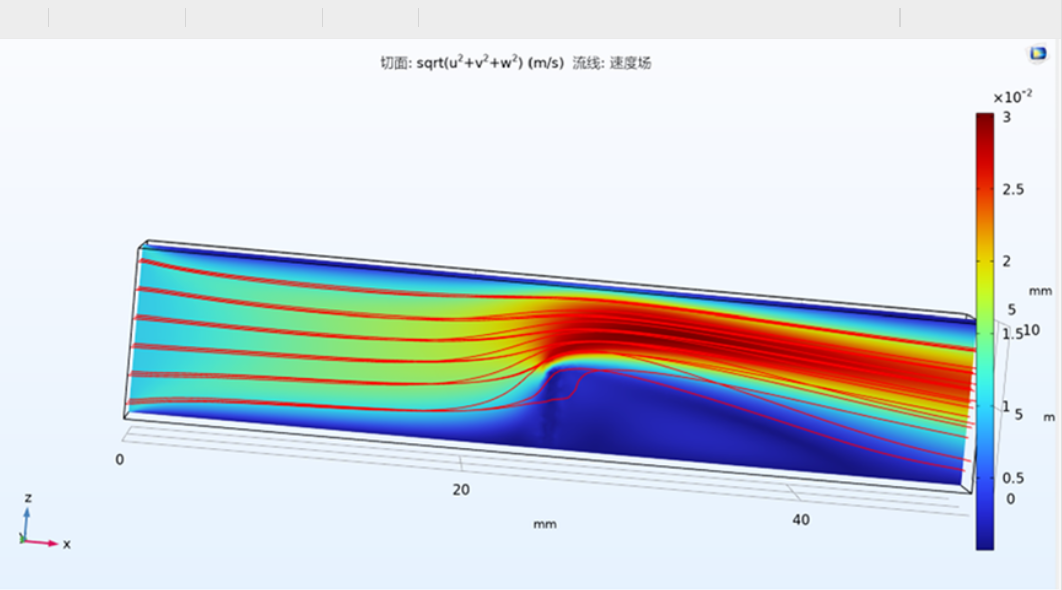
\includegraphics[width=0.45\textwidth]{imgs/youming1}
		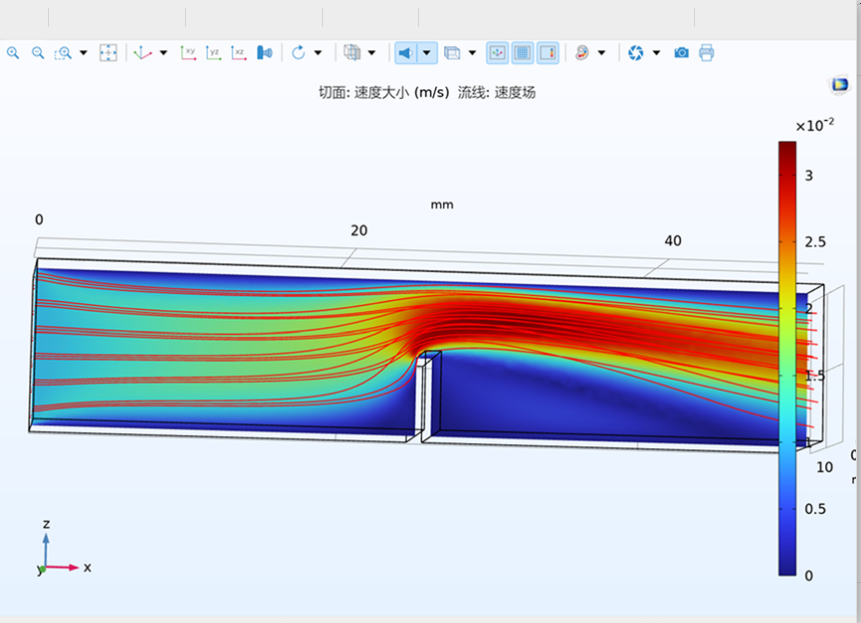
\includegraphics[width=0.45\textwidth]{imgs/youming2}
		
		\textbf{Note:} All figures in this presentation are slices from 3D models.  
		
	\end{frame}

	\begin{frame}{Channel separation}
		Critical to the performance of the model is that the two channels are adequately separated, i.e. that there is no flow between the two fluids. 
		
		Simply implementing the Brinkman method 'as-is' does not separate the channels enough. 
		
		\begin{center}
			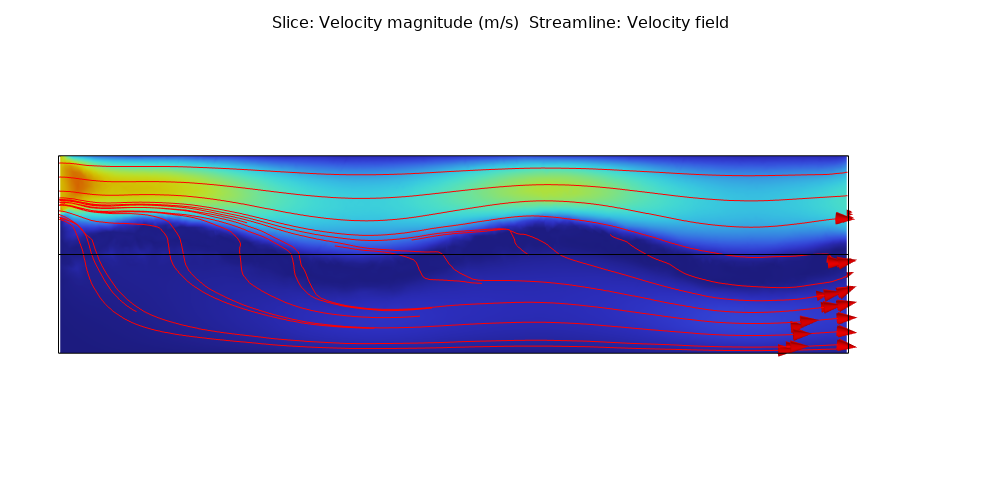
\includegraphics[width=0.45\textwidth]{imgs/separation_failed}
			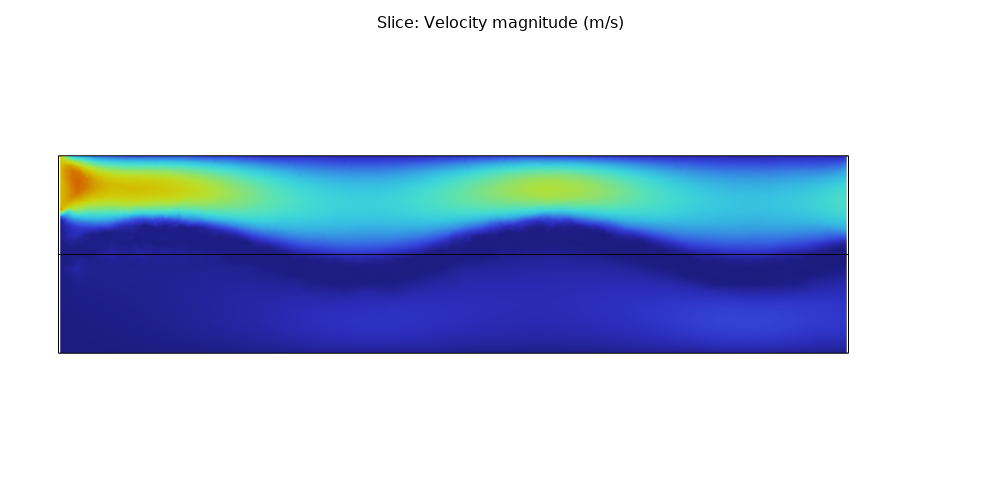
\includegraphics[width=0.45\textwidth]{imgs/separation_failed2.png}
			\sad
		\end{center}
		
		\begin{equation*}
			\text{Solid region: }|z-0.05-0.01\sin(10\pi x)|<0.005
		\end{equation*}
	\end{frame}
	
	\begin{frame}{Single channel}
		For a single channel we can define \emph{both} the wall and other channel so behave like solids, by changing the solid region to:
		\begin{equation*}
		z-0.05-0.01\sin(10\pi x)<0.005. 
		\end{equation*}
		This renders:
		
		\centering
		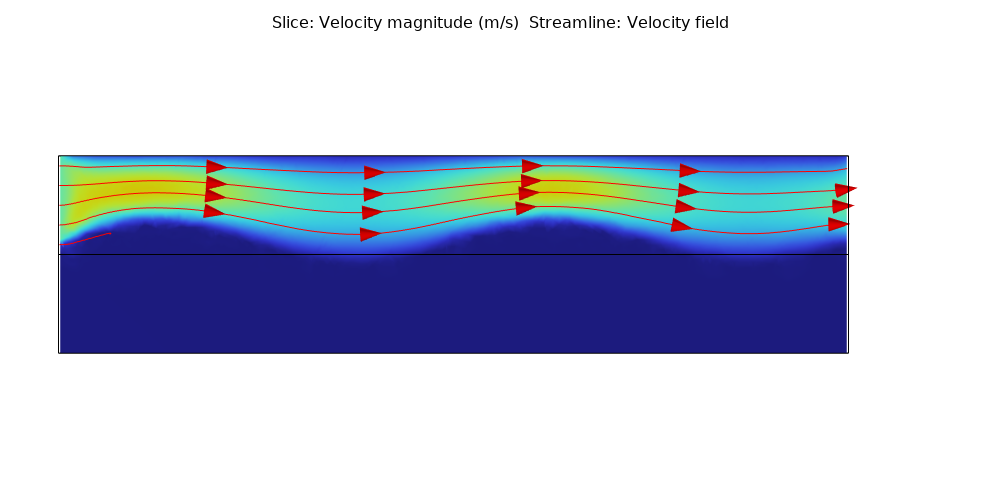
\includegraphics[width=0.9\textwidth]{imgs/sep_1ch_sl}
		\happy
	\end{frame}
	\begin{frame}{Dual channels}
		Luckily the Comsol framework can be nicely adjusted to incorporate two channels in the same model:
		
		\centering
		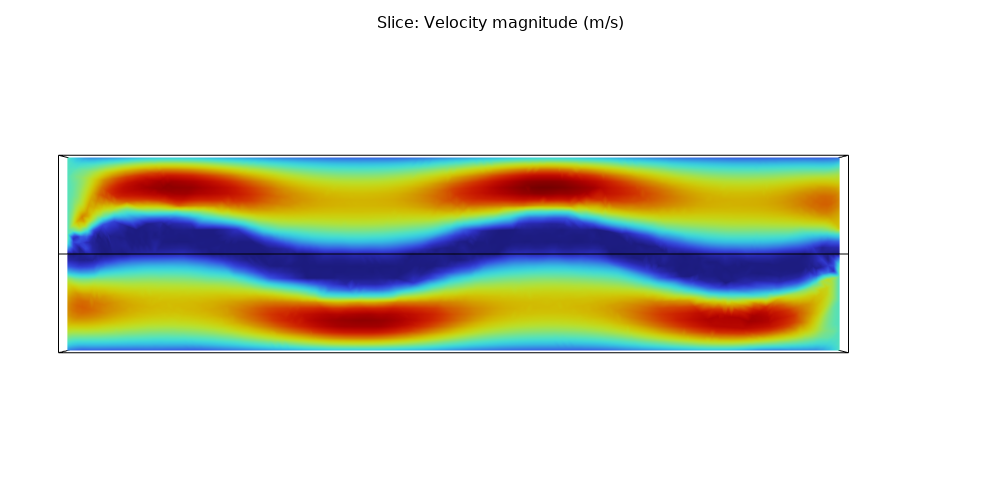
\includegraphics[width=0.49\textwidth]{imgs/sep_2ch}
		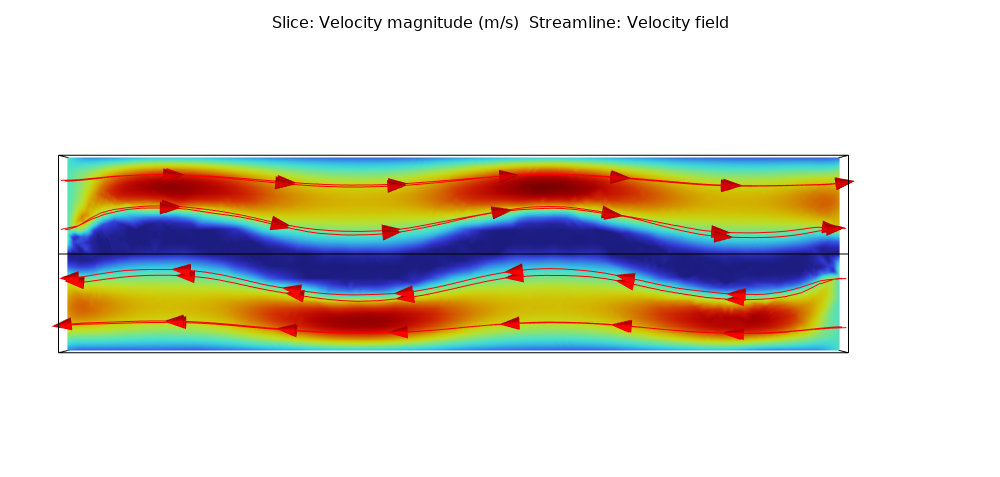
\includegraphics[width=0.49\textwidth]{imgs/sep_2ch_sl}
		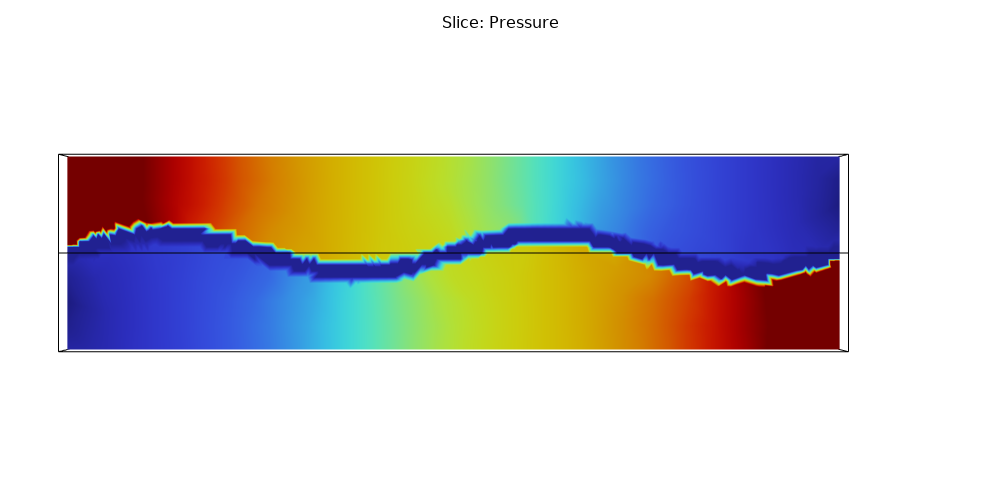
\includegraphics[width=0.49\textwidth]{imgs/sep_2ch_p}
		\begin{align*}
			z-0.05-0.01\sin(10\pi x)&<0.005 \tag{Upper channel} \\
			z-0.05-0.01\sin(10\pi x)&>-0.005 \tag{Lower channel}
		\end{align*}
		
	\end{frame}
	\begin{frame}{Heat transfer}
		Using the same model as before we can turn on the \emph{Heat Transfer in Fluids} module and solve for the temperature distribution. The thermal conductivity is set to \qty{0.6}{\W\per\m\per\K} for water and \qty{400}{\W\per\m\per\K} for copper. From this we can see that the current design of the heat exchanger is very poor:
		
		\centering
		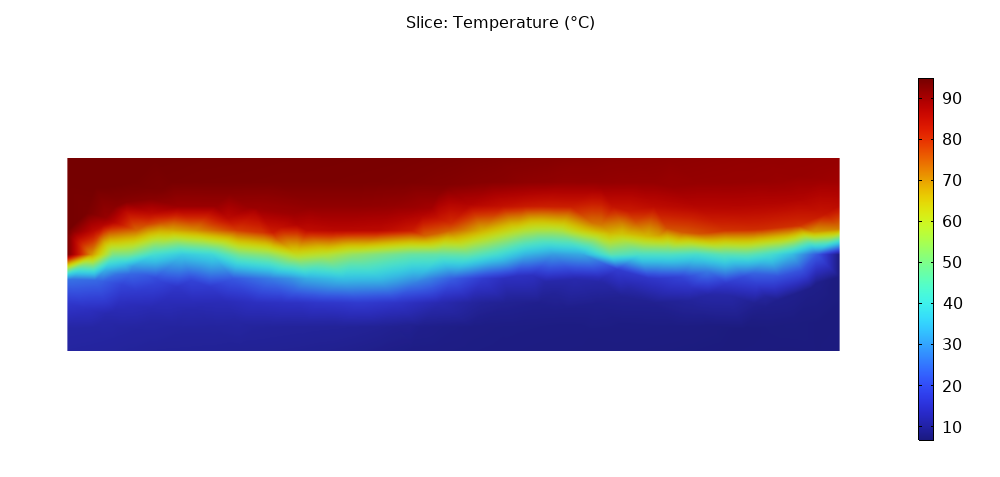
\includegraphics[width=0.7\textwidth]{imgs/sep_2ch_T}
	\end{frame}
\section{TPMS Model}
	\begin{frame}{Background}
		\emph{Triply Periodic Minimal Surfaces} (TPMS) incorporates a wide range of surfaces, of which the \emph{gyroid} is the subject of this project. Discovered by NASA scientist Alan Schoen in 1970, it was proven to be embedded by Grosse-Brauckmann and Wohlgemuth in 1996 \cite{enwiki:gyroid}.
		\begin{itemize}
			\item Embedded; divides space into two \emph{disjoint} sub-volumes. \pause
			\item Can be approximated a the relatively simple equation
			\begin{equation*}
				\sin x\cos y+\sin y\cos z+\sin z\cos x=0
			\end{equation*}
		\end{itemize}\pause
		\centering
		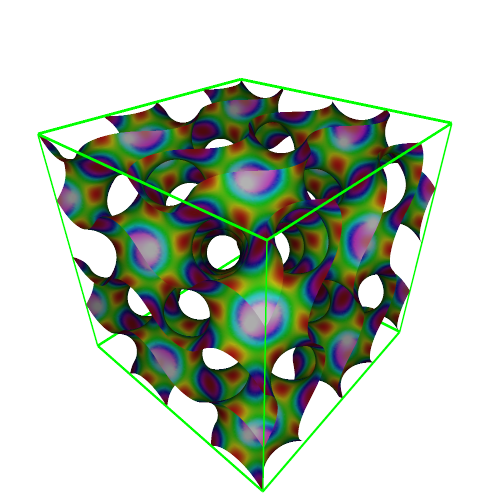
\includegraphics[scale=0.2]{imgs/Gyroid_surface_with_Gaussian_curvature}
		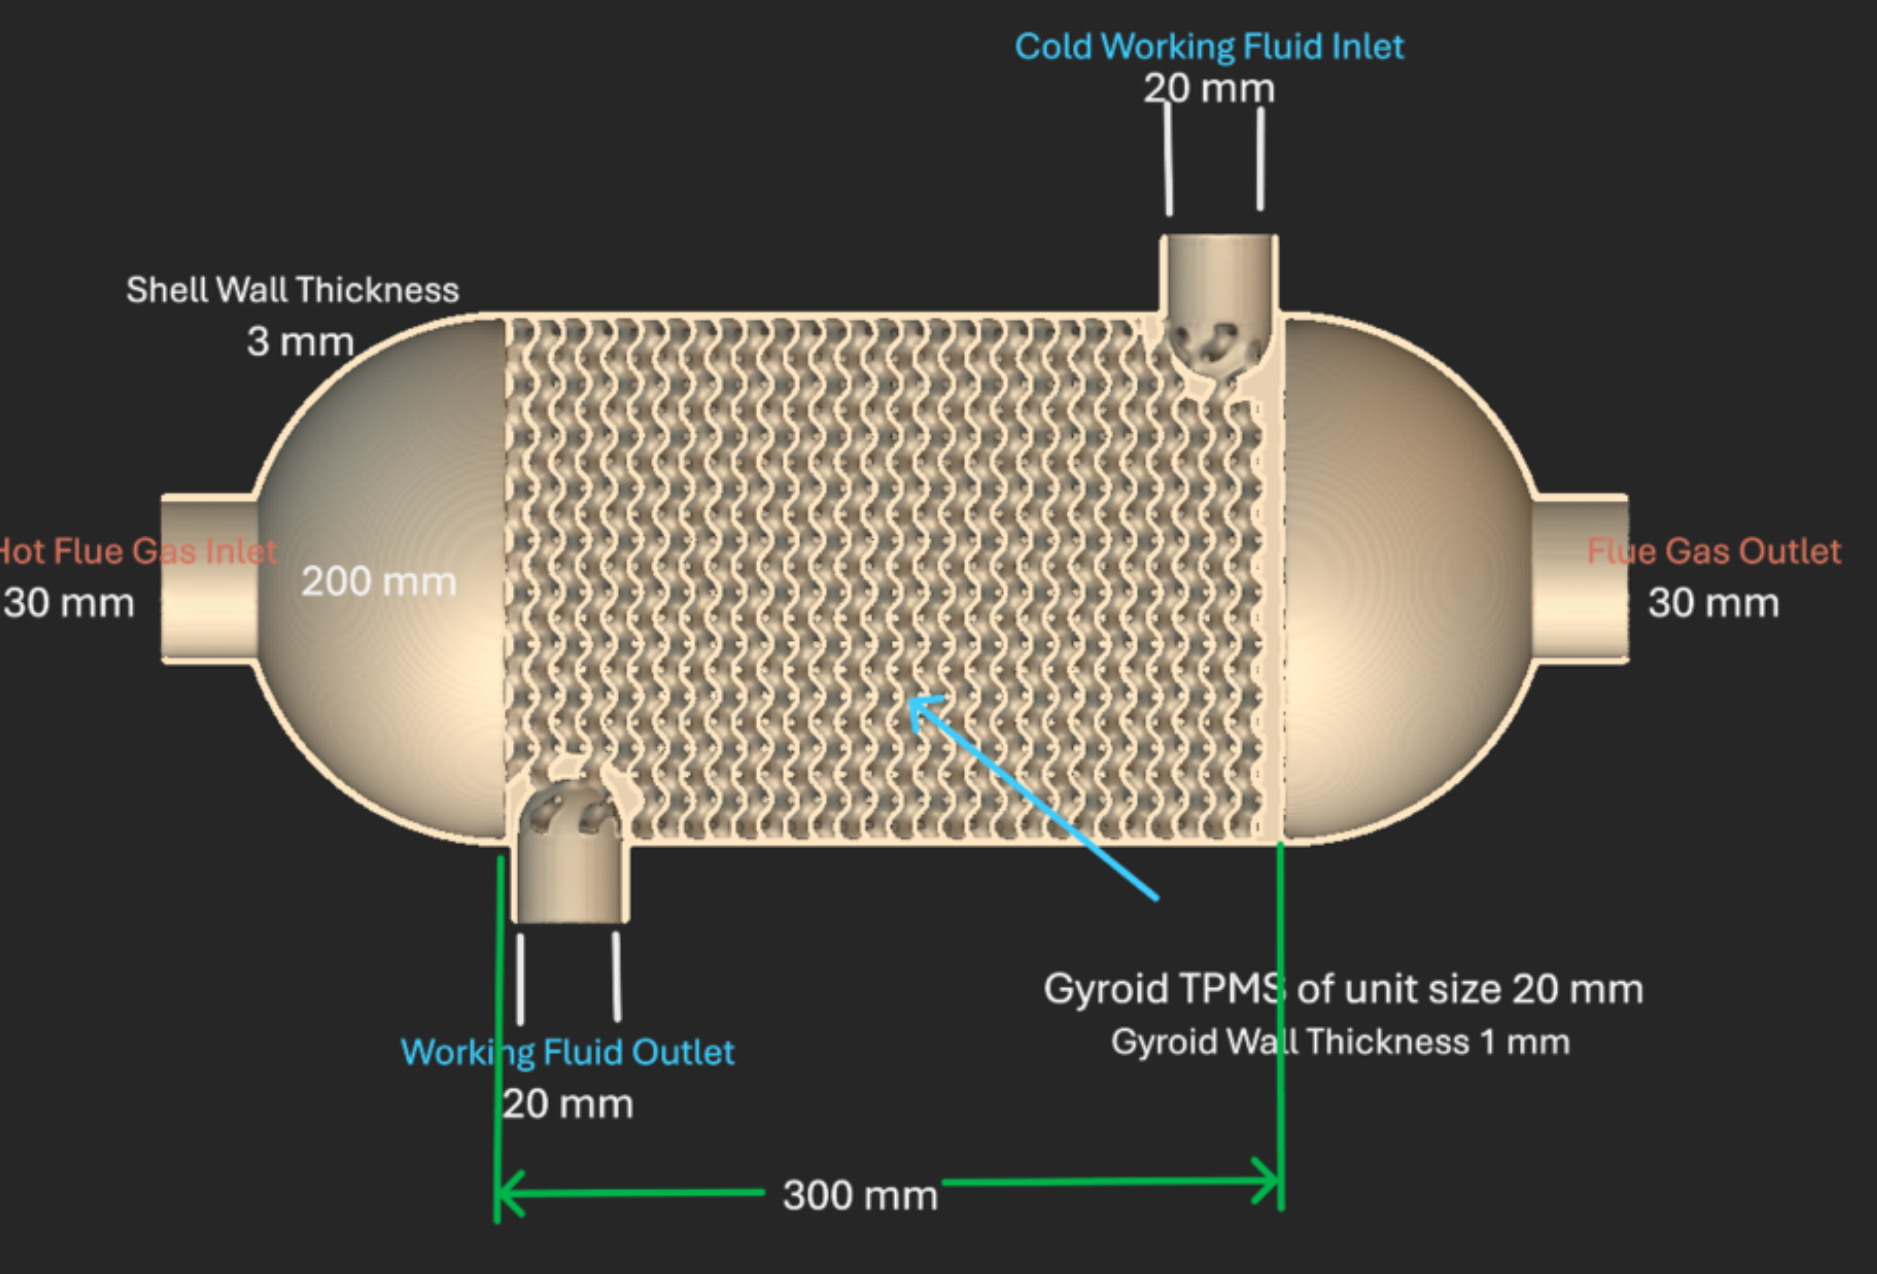
\includegraphics[scale=0.1]{imgs/gyroid_exchanger}
	\end{frame}
	
	\begin{frame}{Advantages of TMPS}
	TPMS provides a compelling alternative to traditional fin-based heat exchangers. 
	\begin{itemize}
		\item High surface-to-volume ratio improves heat exchange.\pause
		\item Continous TPMS walls generally provide good structural integrity (high stiffness).\pause
		\item Geometry can be fine-tuned by function-based parameters. \pause
		\item \emph{Disadvantage:} Difficult to simulate performance
	\end{itemize}
	\end{frame}
\section{References}
	\begin{frame}[allowframebreaks]
		\bibliography{ref.bib}
		\bibliographystyle{alpha}
	\end{frame}
\end{document}
